\documentclass[12pt,a4paper]{article}
\usepackage[margin=0.8in]{geometry}
\usepackage{times}
\usepackage{graphicx}
\usepackage{array}
\usepackage{booktabs}
\usepackage{float}
\usepackage{fancyhdr}
\usepackage{tikz}
\usetikzlibrary{shapes,arrows}

% Header and Footer
\pagestyle{fancy}
\fancyhf{}
\lhead{\fontsize{10}{12}\selectfont MEASUREMENT AND INSTRUMENTATION LABORATORY (ELE 3162)}
\rhead{}
\cfoot{\thepage}
\renewcommand{\headrulewidth}{0.5pt}
\renewcommand{\footrulewidth}{0.5pt}

% Font settings
\renewcommand{\familydefault}{\rmdefault}

\begin{document}

% Title Section
\begin{center}
\fontsize{10}{12}\selectfont \textbf{MEASUREMENT AND INSTRUMENTATION LABORATORY (ELE 3162)}

\vspace{3pt}

\textbf{JAN – MAY 2025}

\vspace{6pt}

\framebox{\textbf{MINI PROJECT}}

\vspace{3pt}

\framebox{\textbf{REVIEW 1: SYNOPSIS}}
\end{center}

\vspace{12pt}

% Problem Statement Box
\noindent
\framebox[1.0\width]{%
\parbox{0.98\textwidth}{%
\textit{``Design a system-level thermal profiling solution using an array of temperature sensors to monitor spatial temperature distribution and generate heat maps. The system enables real-time detection of hotspots and abnormal thermal behaviour to enhance public health and safety. It supports preventive action against overheating, fire hazards, and equipment failure in critical environments. The solution considers societal and environmental aspects by reducing energy loss and improving system reliability. Practical limitations such as sensor accuracy, resolution, cost, and environmental interference are also considered.''}
}
}

\vspace{12pt}

% Project Title
\begin{center}
\colorbox{cyan}{\textbf{Thermal Profiling and Heat Map Generation Using a Temperature Sensor Array}}
\end{center}

\vspace{12pt}

% Students Group
\noindent
\textbf{STUDENTS' GROUP:}

\vspace{8pt}

\begin{table}[H]
\centering
\begin{tabular}{|c|c|c|c|c|}
\hline
\textbf{Sl. no.} & \textbf{Batch} & \textbf{Roll no.} & \textbf{Reg. no.} & \textbf{Full name} \\
\hline
1 & B2 & 39 & 230906310 & T Sreekar Gopal \\
\hline
2 & B2 & 54 & 230906450 & Gonugondla Veera Manikanta \\
\hline
3 & B2 & 65 & 230906510 & Meenakshi Rajeev \\
\hline
\end{tabular}
\end{table}

\vspace{12pt}

% Objectives
\noindent
\textbf{OBJECTIVES:}

\vspace{8pt}

\begin{enumerate}
\item To measure spatial temperature distribution using an array of temperature sensors
\item To generate heat maps for visual representation of thermal profiles.
\item To detect thermal abnormalities such as hotspots through continuous monitoring.
\item To develop firmware for microcontroller-based data acquisition and transmission via industrial protocols.
\item To implement machine learning algorithms for anomaly detection and predictive maintenance.
\end{enumerate}

\vspace{12pt}
\newpage


% Flowchart Section
\noindent
\textbf{FLOWCHART SHOWING METHODOLOGY:}

\vspace{12pt}

\begin{center}
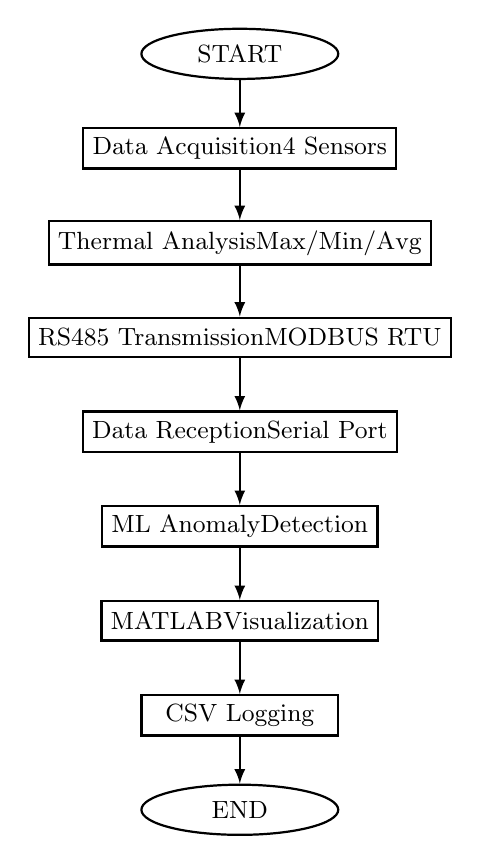
\begin{tikzpicture}[node distance=1.2cm, every node/.style={draw, thick, minimum width=2.5cm, minimum height=0.5cm, text centered, font=\small}]

% Define styles
\tikzstyle{startstop} = [ellipse, fill=white, draw=black]
\tikzstyle{process} = [rectangle, fill=white, draw=black]
\tikzstyle{arrow} = [thick, ->, >=latex]

% Nodes
\node[startstop] (start) {START};

\node[process, below of=start] (acq) {Data Acquisition\\4 Sensors};
\draw[arrow] (start) -- (acq);

\node[process, below of=acq] (analysis) {Thermal Analysis\\Max/Min/Avg};
\draw[arrow] (acq) -- (analysis);

\node[process, below of=analysis] (rs485) {RS485 Transmission\\MODBUS RTU};
\draw[arrow] (analysis) -- (rs485);

\node[process, below of=rs485] (recv) {Data Reception\\Serial Port};
\draw[arrow] (rs485) -- (recv);

\node[process, below of=recv] (ml) {ML Anomaly\\Detection};
\draw[arrow] (recv) -- (ml);

\node[process, below of=ml] (viz) {MATLAB\\Visualization};
\draw[arrow] (ml) -- (viz);

\node[process, below of=viz] (log) {CSV Logging};
\draw[arrow] (viz) -- (log);

\node[startstop, below of=log] (end) {END};
\draw[arrow] (log) -- (end);

\end{tikzpicture}
\end{center}



% Justification Section
\noindent
\textbf{JUSTSIFICATION AS PER THE PROBLEM STATEMENT (Public health and safety, and cultural, societal, and environmental considerations):}

\vspace{12pt}

\begin{enumerate}

\item \textbf{\underline{Public Health and Safety:}} Continuous thermal monitoring and early detection of hotspots help prevent fire accidents, overheating of equipment, and unsafe working conditions, thereby protecting human life and public infrastructure.

\vspace{8pt}

\item \textbf{\underline{Societal and Environmental Considerations:}} By enabling efficient thermal management and early fault identification, the system reduces energy wastage, minimizes environmental impact, and promotes sustainable and responsible use of electrical and industrial systems.

\vspace{8pt}

\item \textbf{\underline{Understanding of Limitations:}} The system design accounts for limitations such as sensor placement density, measurement accuracy, response delays, and cost, ensuring a balanced, scalable, and practical solution suitable for real-world deployment.

\end{enumerate}

\vspace{12pt}
\newpage
% Software Section
\noindent
\textbf{SOFTWARE:}

\vspace{8pt}

\begin{table}[H]
\centering
\begin{tabular}{|c|l|p{6cm}|}
\hline
\textbf{Sl. No.} & \textbf{Software} & \textbf{Purpose} \\
\hline
1. & Arduino IDE & Programming the controller for temperature data acquisition from DS18B20 sensors and transmitting data via RS-485. \\
\hline
2. & Serial Monitoring Software (Arduino Serial Monitor) & Receiving and monitoring real-time temperature data from the RS-485 network. \\
\hline
3. & MATLAB / Python & Processing temperature data and generating heat maps for thermal profiling and hotspot detection. \\
\hline
\end{tabular}
\end{table}

\vspace{12pt}

% Hardware Section
\noindent
\textbf{HARDWARE COMPONENTS AND TENTATIVE BILL OF MATERIALS:}

\vspace{8pt}

\begin{table}[H]
\centering
\begin{tabular}{|c|l|c|}
\hline
\textbf{Sl. No.} & \textbf{Component} & \textbf{Approx. cost} \\
\hline
1. & DS18B20 Waterproof Digital Temperature Sensor (Qty: 4) & Rs. 912 \\
\hline
2. & MAX485 RS-485 TTL Module (Qty: 2) & Rs. 114 \\
\hline
3. & USB to RS-485 Converter Programmer Module (CH340C Chipset) & Rs. 368 \\
\hline
4. & ESP32 Development Board & Rs. 450 \\
\hline
5. & Jumper Wires Set, Breadboard, Pull-up Resistors & Rs. 200 \\
\hline
& \textbf{Total expenditure:} & \textbf{Rs. 2,044} \\
\hline
\end{tabular}
\end{table}

\end{document}
